\newpage
\section{插入图片}

%%单张图片插入
\begin{figure}[!htb]
	%其中!h只是试图将图片放在当前位置,如果页面剩下的部分放不下,还是会跑到下一页的(t)顶部或者(b)底部。
	%H借助float包可以固定图片位置
	\centering
	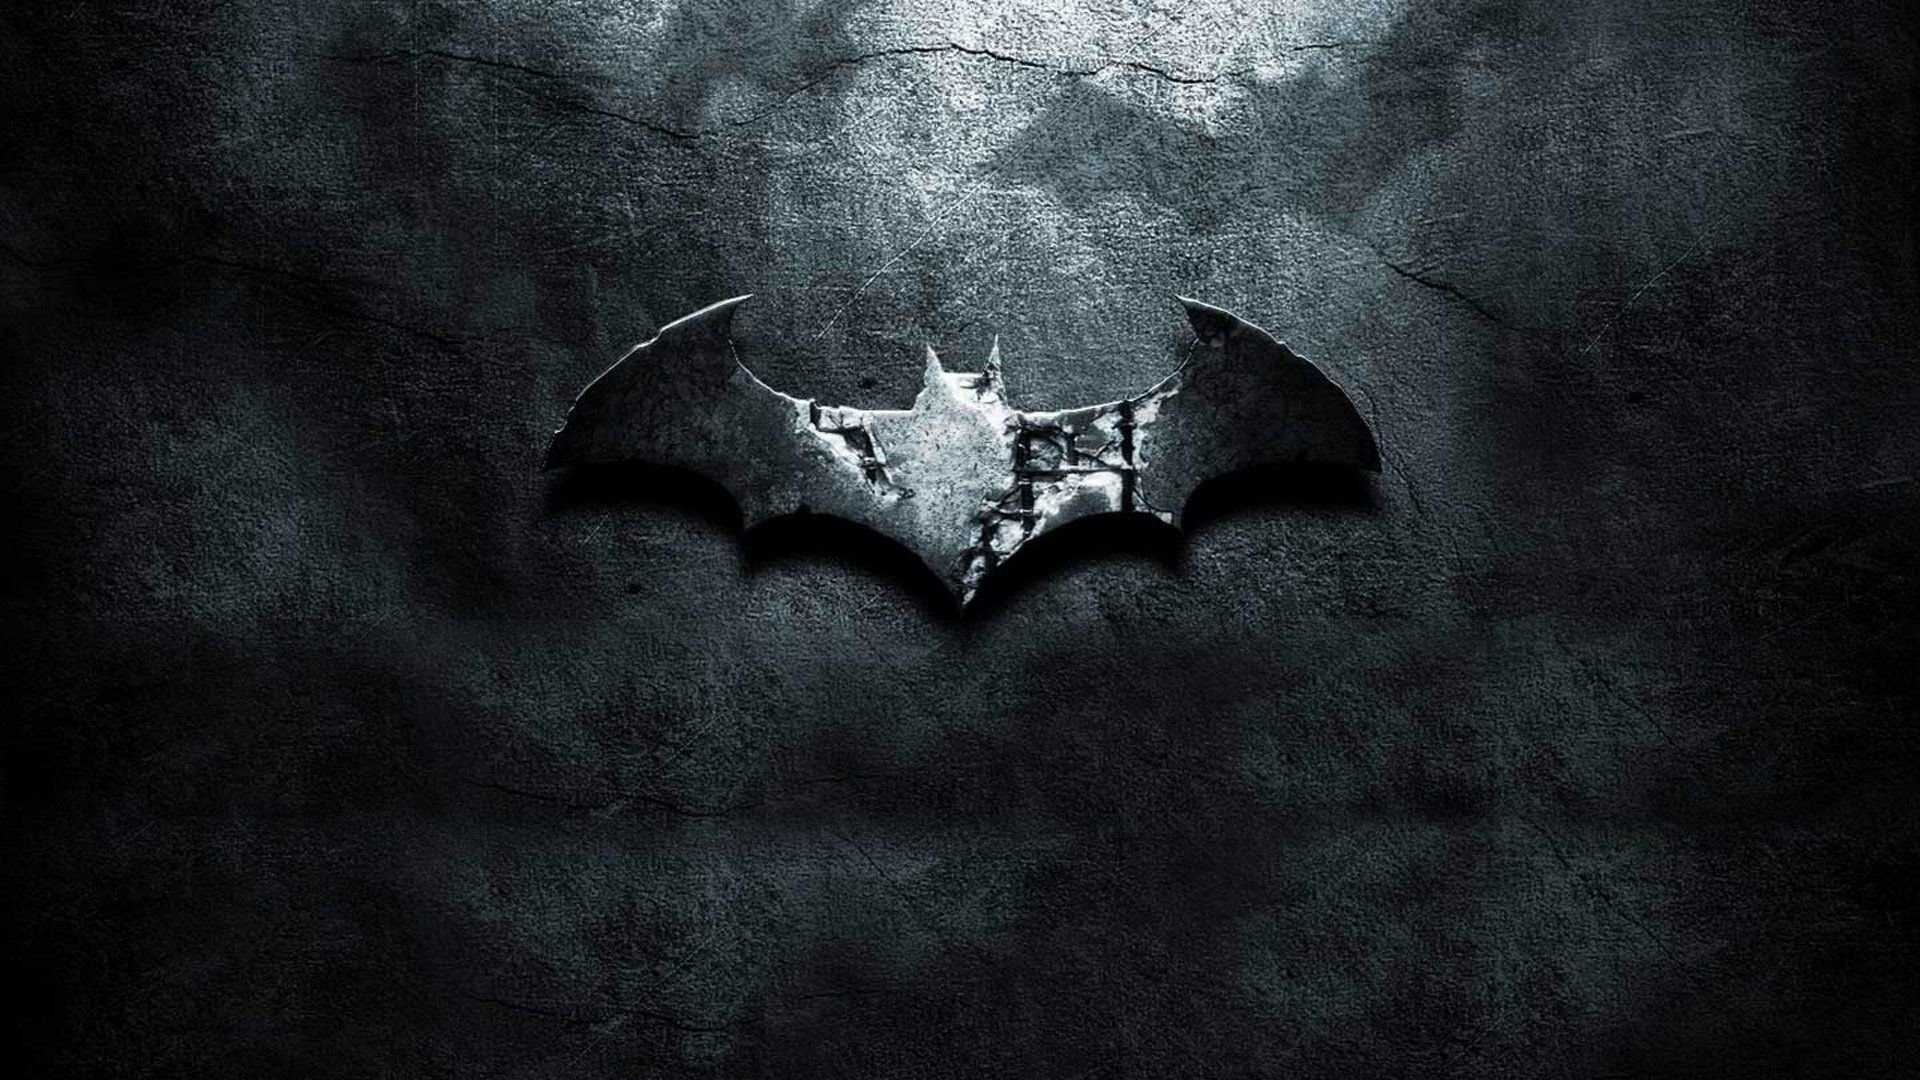
\includegraphics[width = 0.7\linewidth]{./pictures/94.jpg}
	\caption{蝙蝠侠}\label{fig:1}
\end{figure}

%%并排两张图片插入

\begin{figure}[htbp]  %[htbp]中的h是浮动的意思
	\centering    %居中
	\subfloat[蝙蝠侠] %第一张子图
	{
		\begin{minipage}[t]{0.5\textwidth}
			\centering%子图居中
			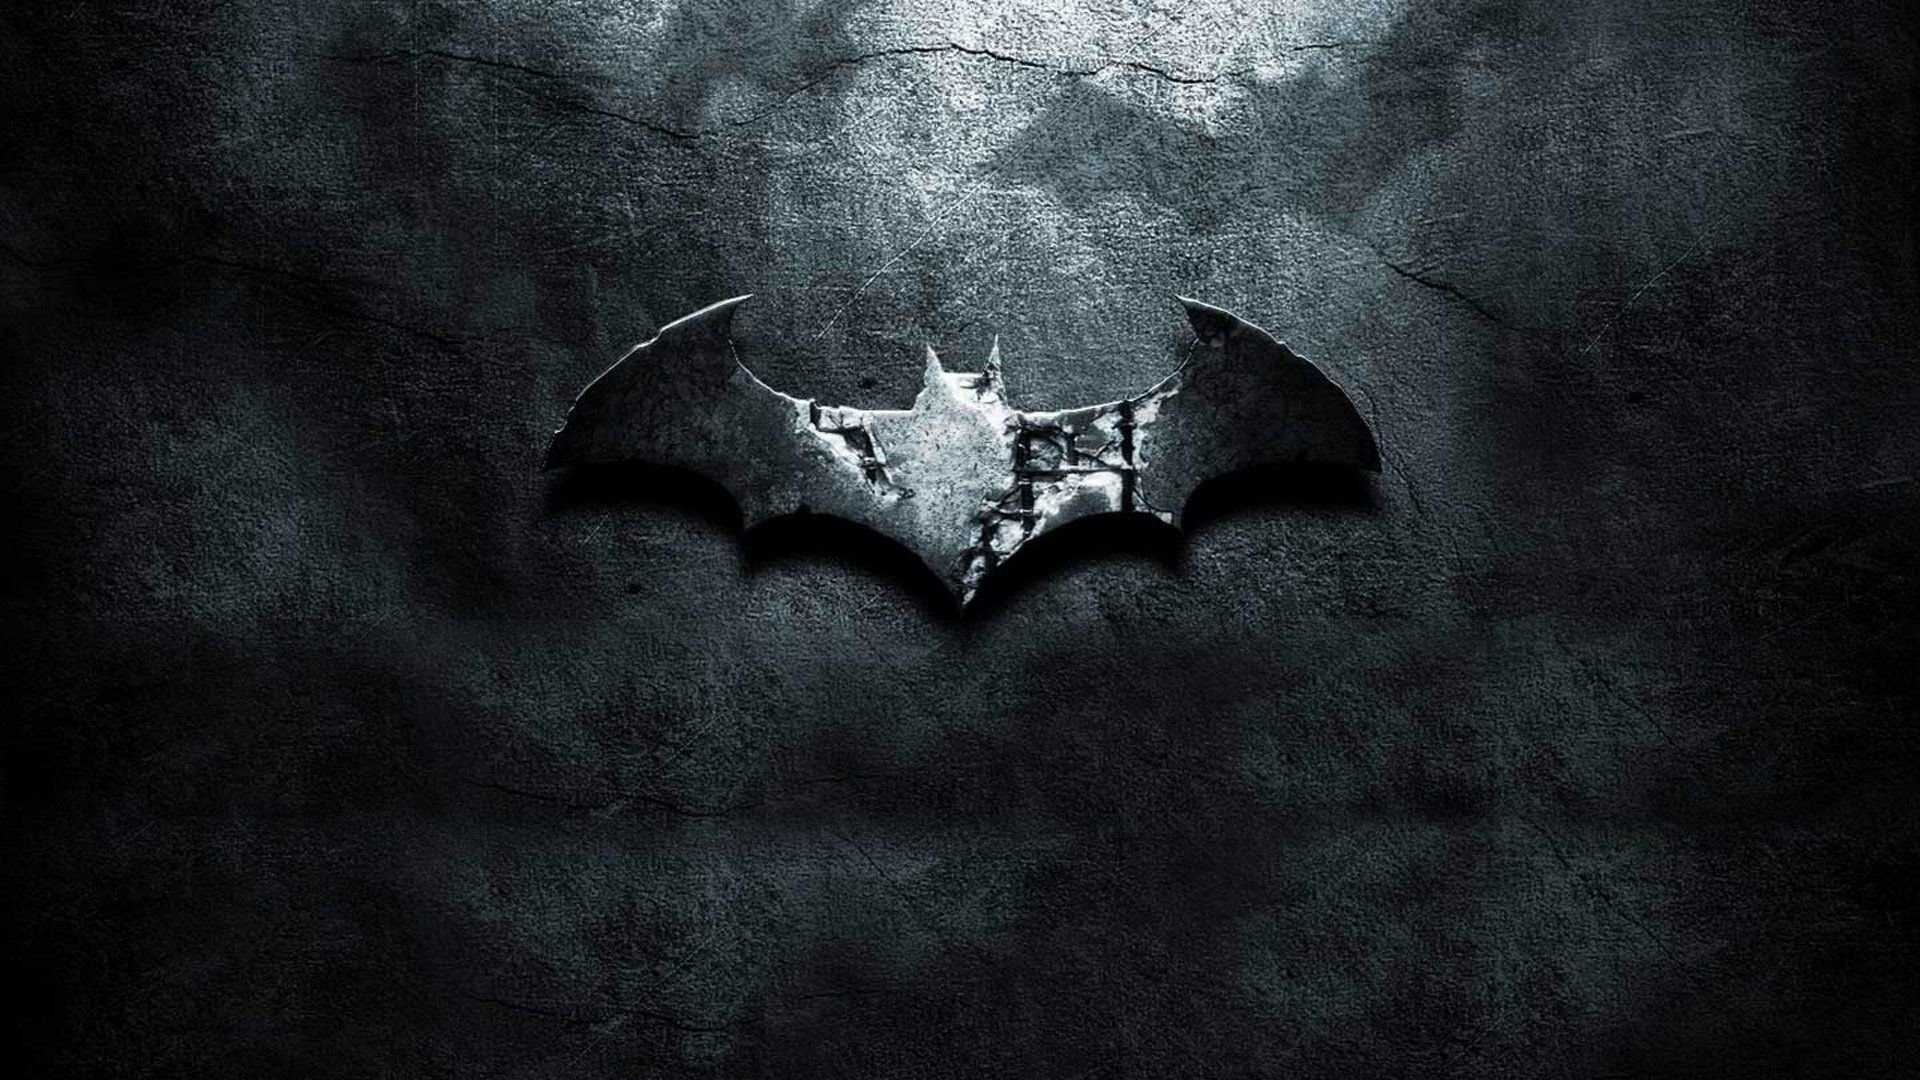
\includegraphics[width=0.65\textwidth]{./pictures/94.jpg}   %以行宽的0.5倍大小显示
			\label{fig1}
		\end{minipage}%
	}%注意这里不能回车空行,否则两张图会上下排列,而不是并排排列
	\subfloat[钢铁侠] %第二张子图
	{
		\begin{minipage}[t]{0.5\textwidth}
			\centering      %子图居中
			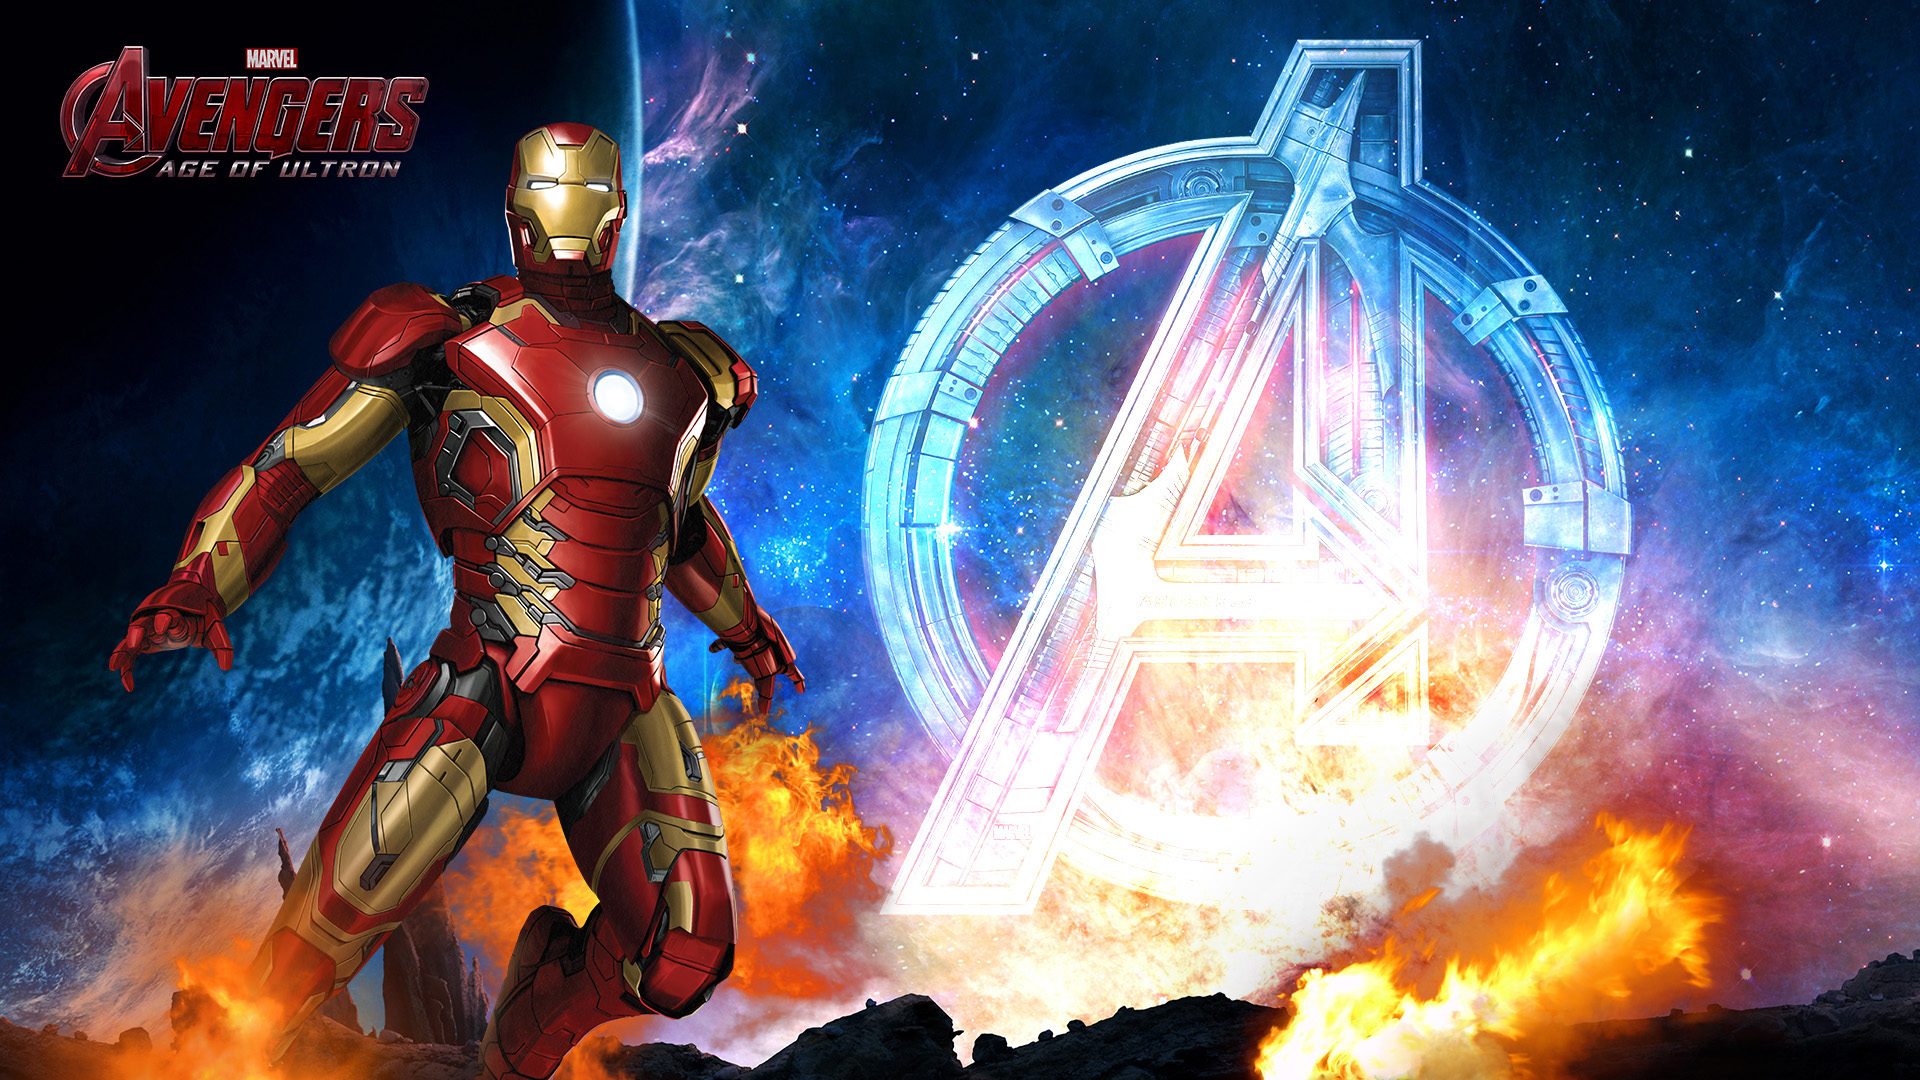
\includegraphics[width=0.65\textwidth]{./pictures/6.jpg}   %以行宽的0.5倍大小显示
			\label{fig2}
		\end{minipage}
	}
	\caption{Schematic diagram of a four-level tripod-type atomic system driven by three coherent laser fields.} %  %大图名称
	\label{FIG}  %图片引用标记
\end{figure}
图片 \ref{fig1} 是蝙蝠侠,图片 \ref{fig2} 是钢铁侠,图片 \ref{FIG} (a)是蝙蝠侠。



%% 插入2*2排列图片,m*n类似,用 \quad 来换行
\begin{figure}[htbp]
	\centering
	\subfloat[SubCaption\_1]
	{
		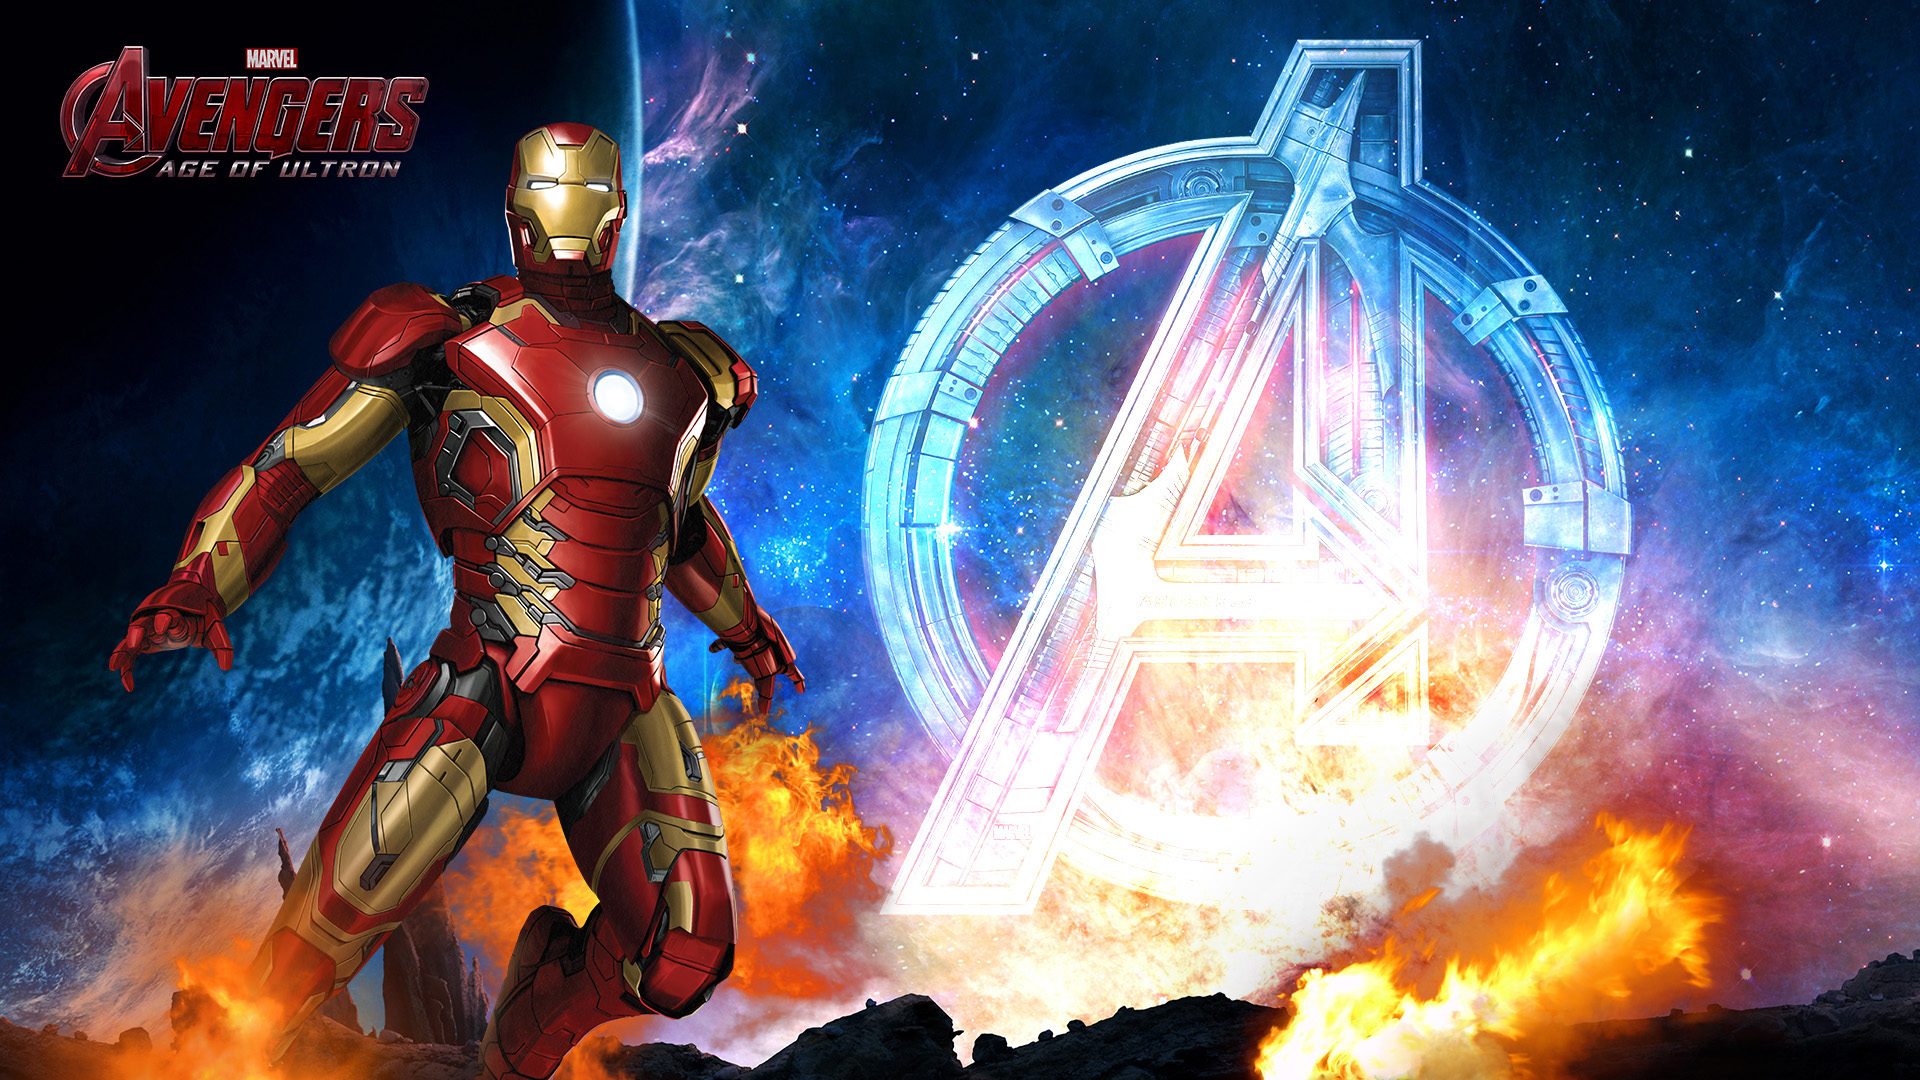
\includegraphics[width=2.5in]{./pictures/6.jpg}
		\label{label_for_cross_ref_1}
	}
	\subfloat[SubCaption\_2]
	{
		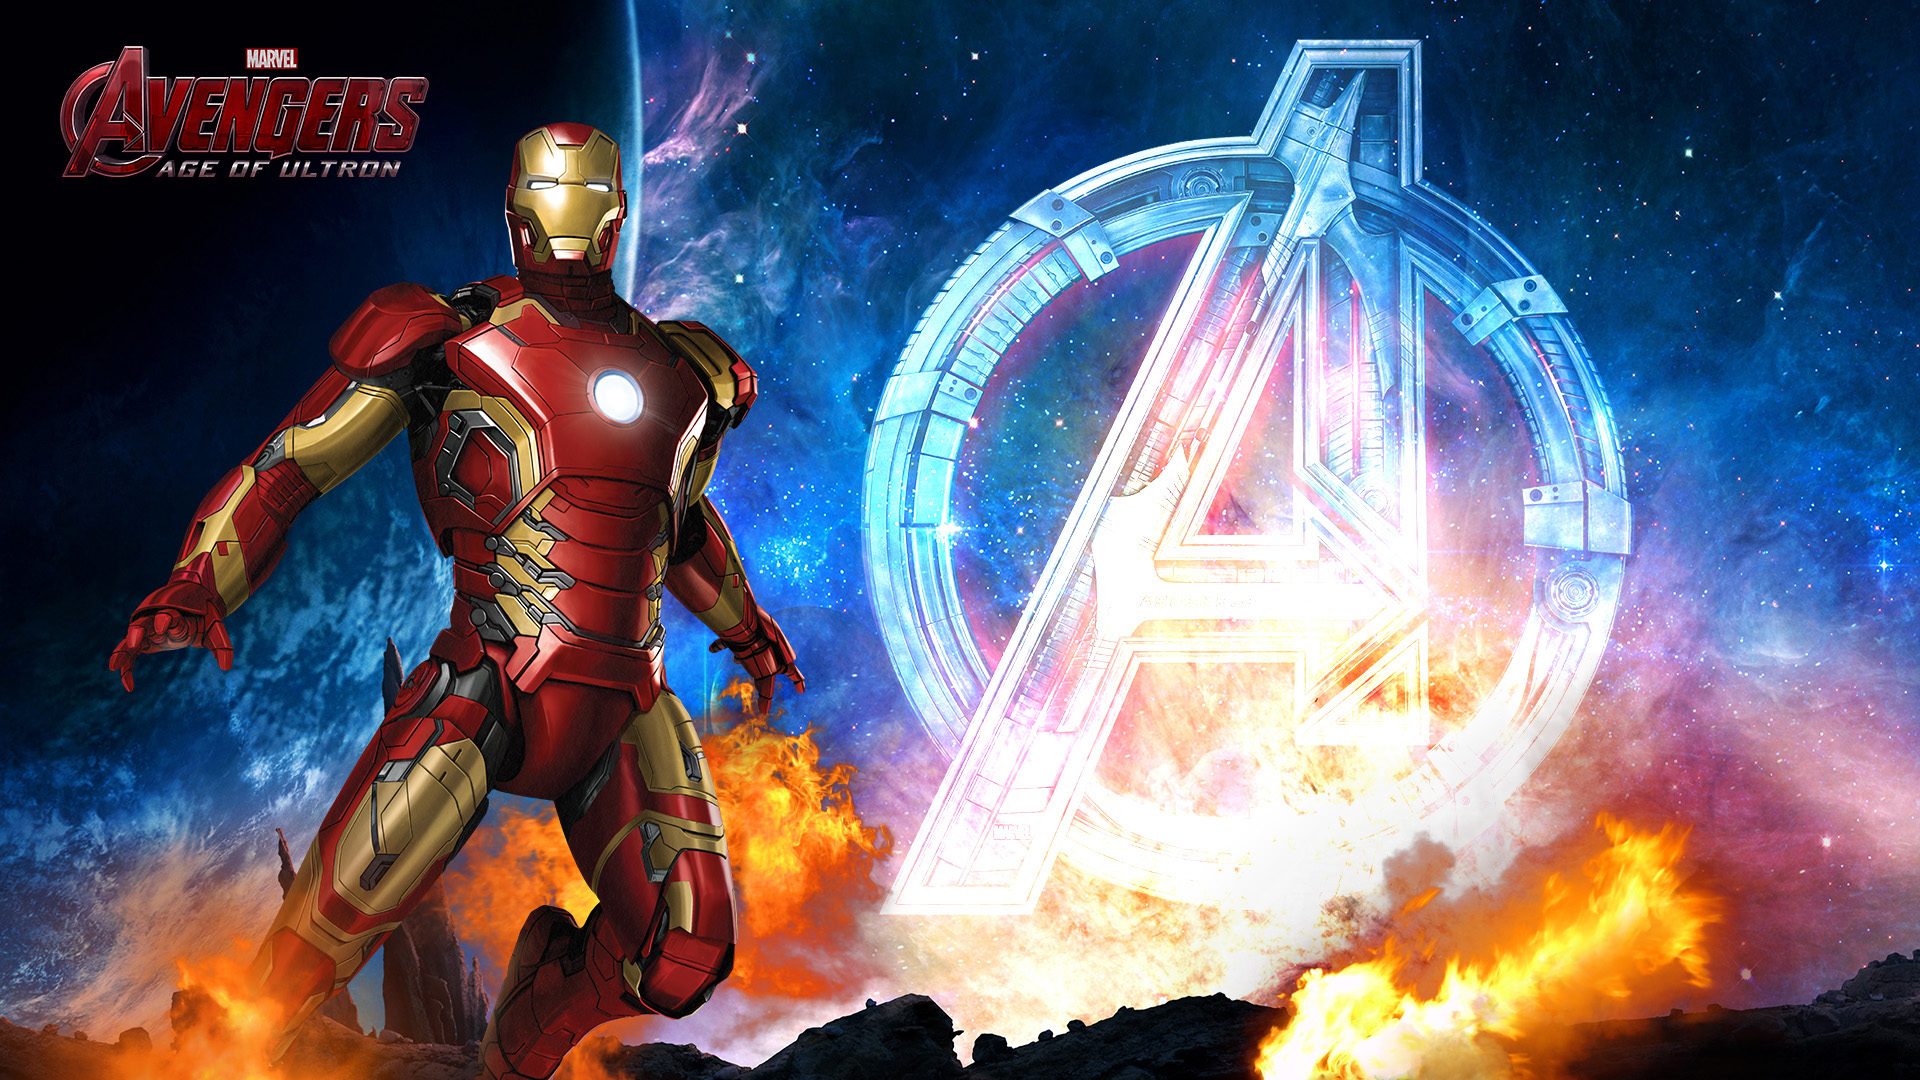
\includegraphics[width=2.5in]{./pictures/6.jpg}
		\label{label_for_cross_ref_2}
	}
	\quad    %用 \quad 来换行
	\subfloat[SubCaption\_3]
	{
		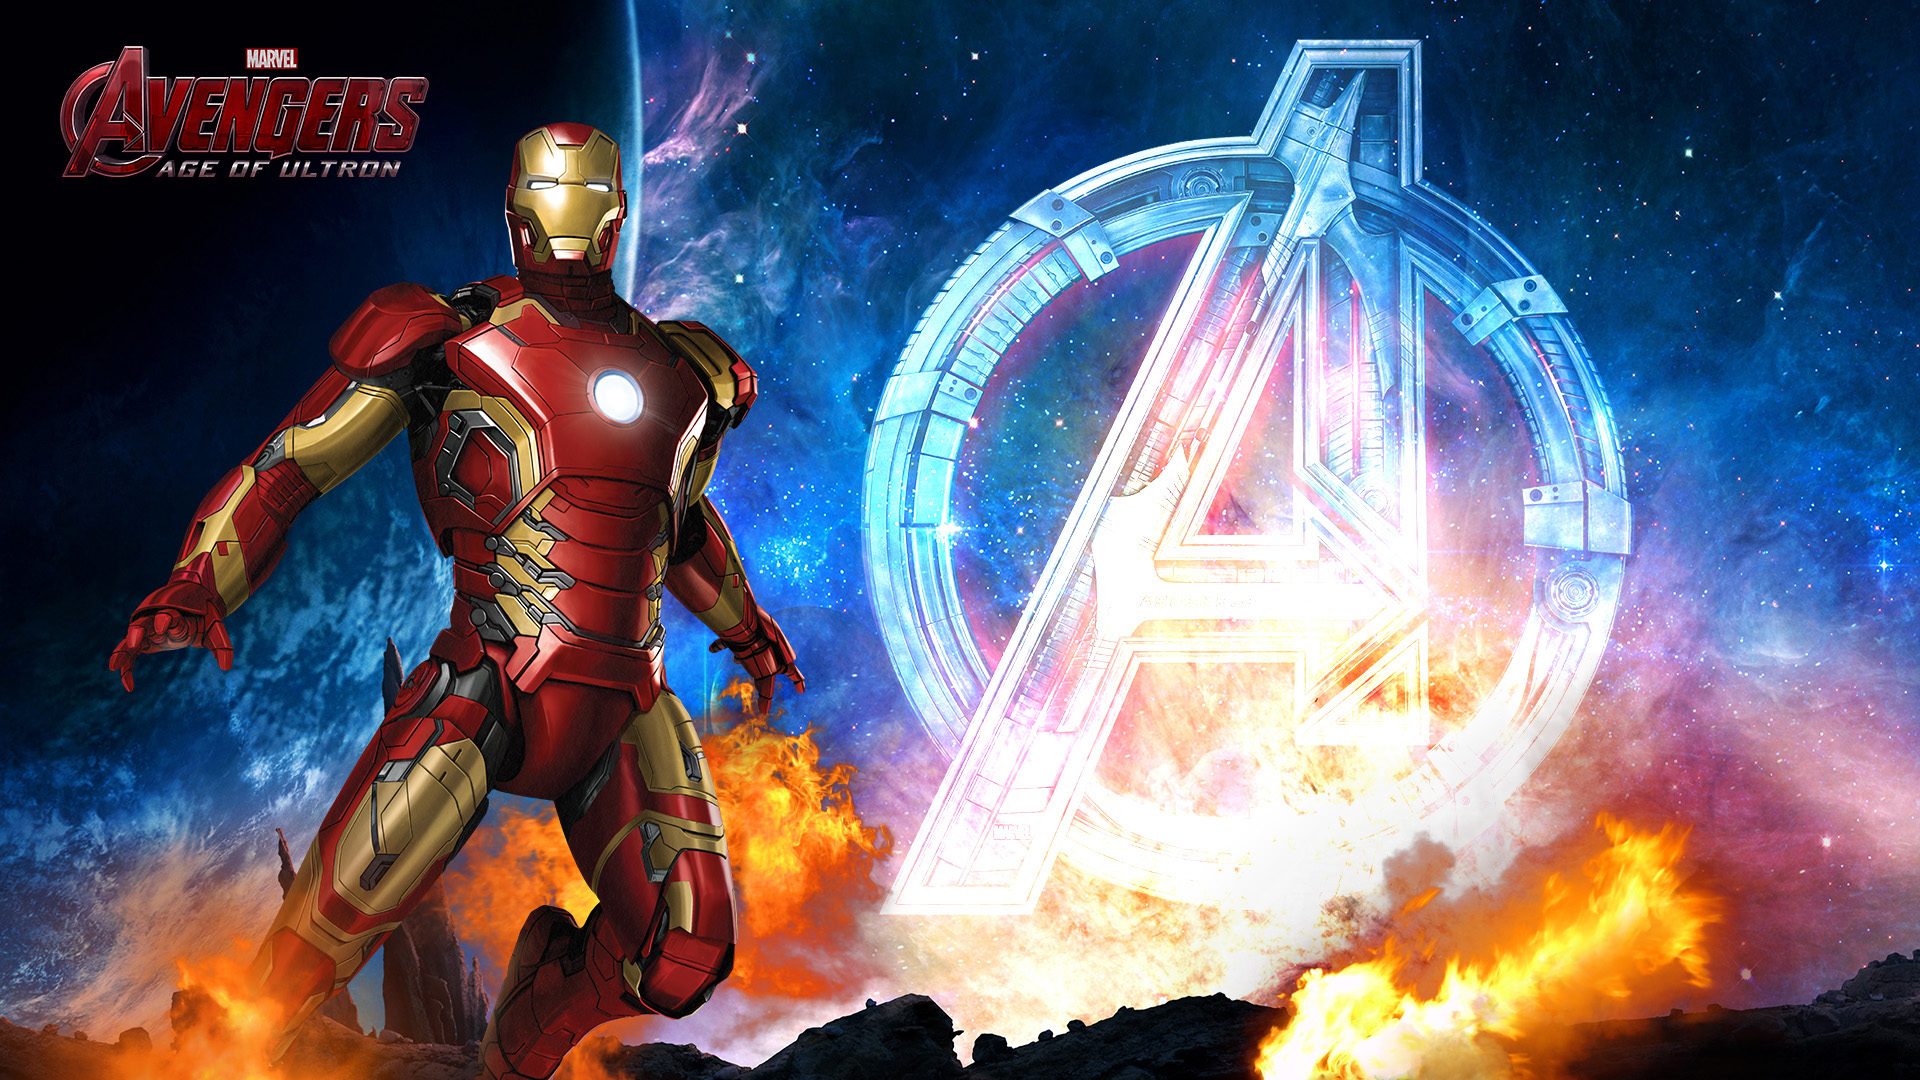
\includegraphics[width=2.5in]{./pictures/6.jpg}
		\label{label_for_cross_ref_3}
	}
	\subfloat[SubCaption\_4]
	{
		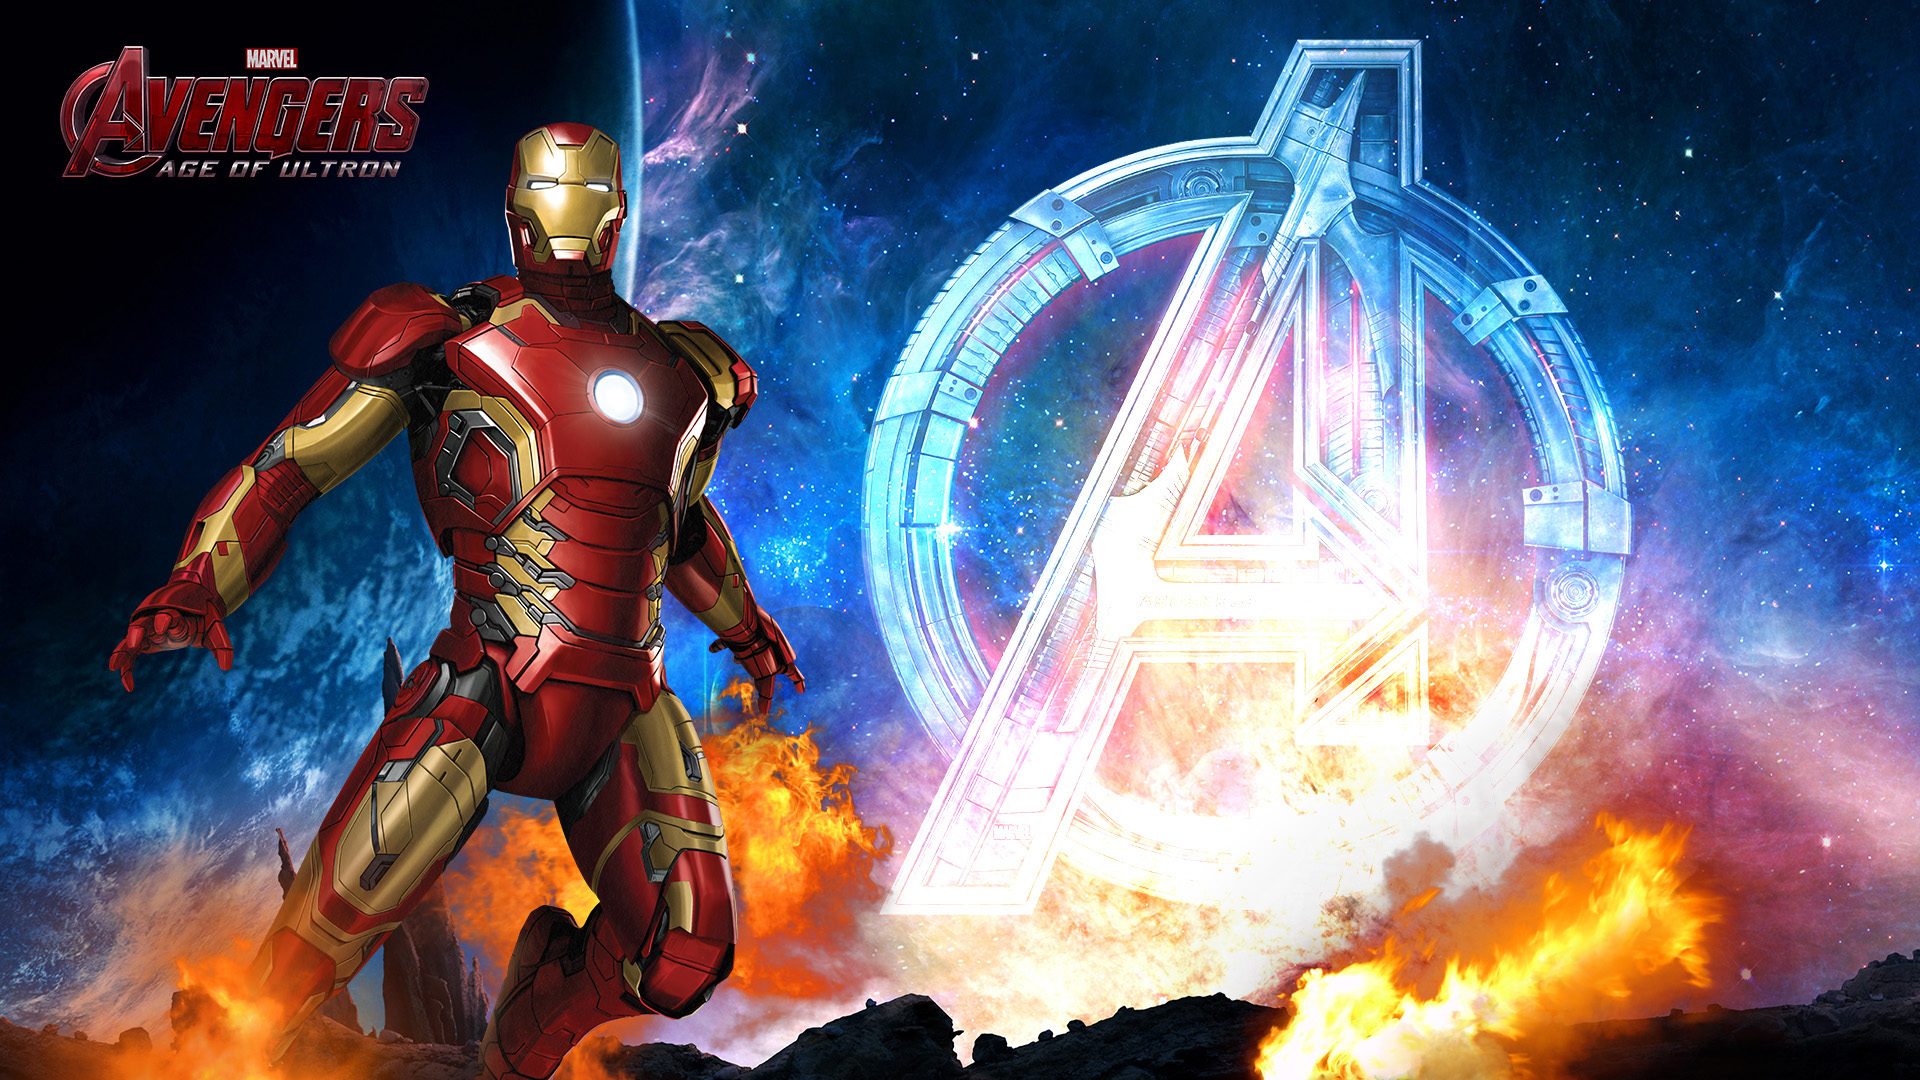
\includegraphics[width=2.5in]{./pictures/6.jpg}
		\label{label_for_cross_ref_4}
	}
	\caption{This is a Demo of $2\times 2$}
	\label{fig.1}
\end{figure}

